\begin{frame}
  \frametitle{Hypothetical (?) scenarios}

  \begin{itemize}
  \item<1-> The computer vision subsystem of an autonomous vehicle leads the
    vehicle to take a left turn, in front of a car moving in the opposite direction\footnote{\url{https://www.theguardian.com/technology/2022/dec/22/tesla-crash-full-self-driving-mode-san-francisco}}
  \item<2-> The credit assessment system leads to the rejection of an
    application for a loan - the client suspects racial bias\footnote{\url{https://www.technologyreview.com/2021/06/17/1026519/racial-bias-noisy-data-credit-scores-mortgage-loans-fairness-machine-learning/}}
  \item<3-> A model that assesses the risk of future criminal offenses (and
    used for decisions on parole sentences) is biased against black
    prisoners\footnote{\url{https://www.propublica.org/article/machine-bias-risk-assessments-in-criminal-sentencing}}
  \end{itemize}

\end{frame}

\begin{frame}
  \frametitle{Questions}
  \begin{itemize}
  \item Why did the model make a specific decision? \textcolor{red}{local XAI}
  \item What could we change so that the model will make a different decision? \textcolor{red}{counterfactual}
  \item Can we summarize the model's behavior? \textcolor{red}{global XAI}
  \item Models as knowledge extractors, what hat the model learnt \textcolor{red}{global XAI}
  \end{itemize}
\end{frame}

\begin{frame}
  \frametitle{Interpretability of Machine Learning Models}
  Qualitative definitions:
  \begin{itemize}
  \item<1-> ``Interpretability is the degree to which a human can understand the
    cause of a decision'' \footnote{Miller, Tim. ``Explanation in artificial
    intelligence: Insights from the social sciences.'' arXiv Preprint
    arXiv:1706.07269. (2017)}
  \item<2-> ``Interpretability is the degree to which a human can consistently
    predict the model’s result''\footnote{Kim, Been, Rajiv Khanna, and
    Oluwasanmi O. Koyejo. ``Examples are not enough, learn to criticize!
    Criticism for interpretability.'' Advances in Neural Information Processing
    Systems (2016).}
  \item<3-> ``Extraction of relevant knowledge from a machine-learning model
    concerning relationships either contained in data or learned by the
    model''\footnote{Murdoch, W. J., Singh, C., Kumbier, K., Abbasi-Asl, R. and
    Yu, B. ``Definitions, methods, and applications in interpretable machine
    learning.'' Proceedings of the National Academy of Sciences, 116(44),
    22071-22080. (2019)}
  \end{itemize}
\end{frame}

\begin{frame}
  \frametitle{My understanding}
  Interpretability is the degree to which a human can understand the reasoning process for a (specific) prediction

  \begin{itemize}
    \item interpretability: either by-design or assisted by a post-hoc XAI technique
    \item degree: non binary, interpretability is a spectrum
    \item human: interpretability is a human-centric procedure
    \item reasoning process: mechanism for predicting
  \end{itemize}
  \end{frame}

\subsection{Global vs Local}

\begin{frame}
  \frametitle{Global vs Local}
  \begin{itemize}
    \item \textcolor{red}{Local}
    \begin{itemize}
      \item Interpret the model's output for a particular input
      \item Extract interpretable quantity that holds for $x$ close to $x^{(i)}$
    \end{itemize}

    \item \textcolor{red}{Global}
    \begin{itemize}
      \item Provide a general interpretation of the model's behavior
      \item Extract interpretable quantity that holds for $x \in \mathcal{X}$
    \end{itemize}
  \end{itemize}

  \begin{figure}
    \centering
    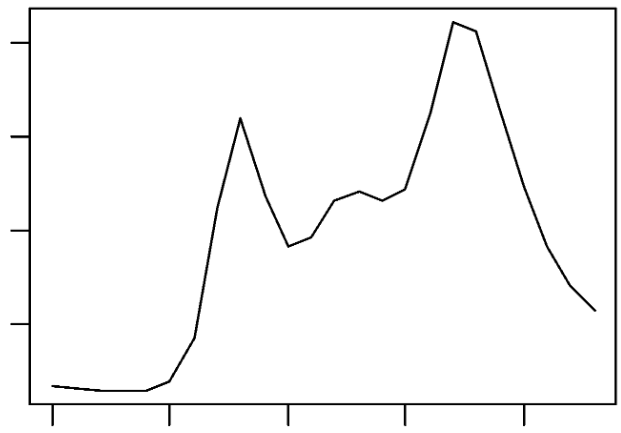
\includegraphics[width=0.37\linewidth]{ale_concept}
    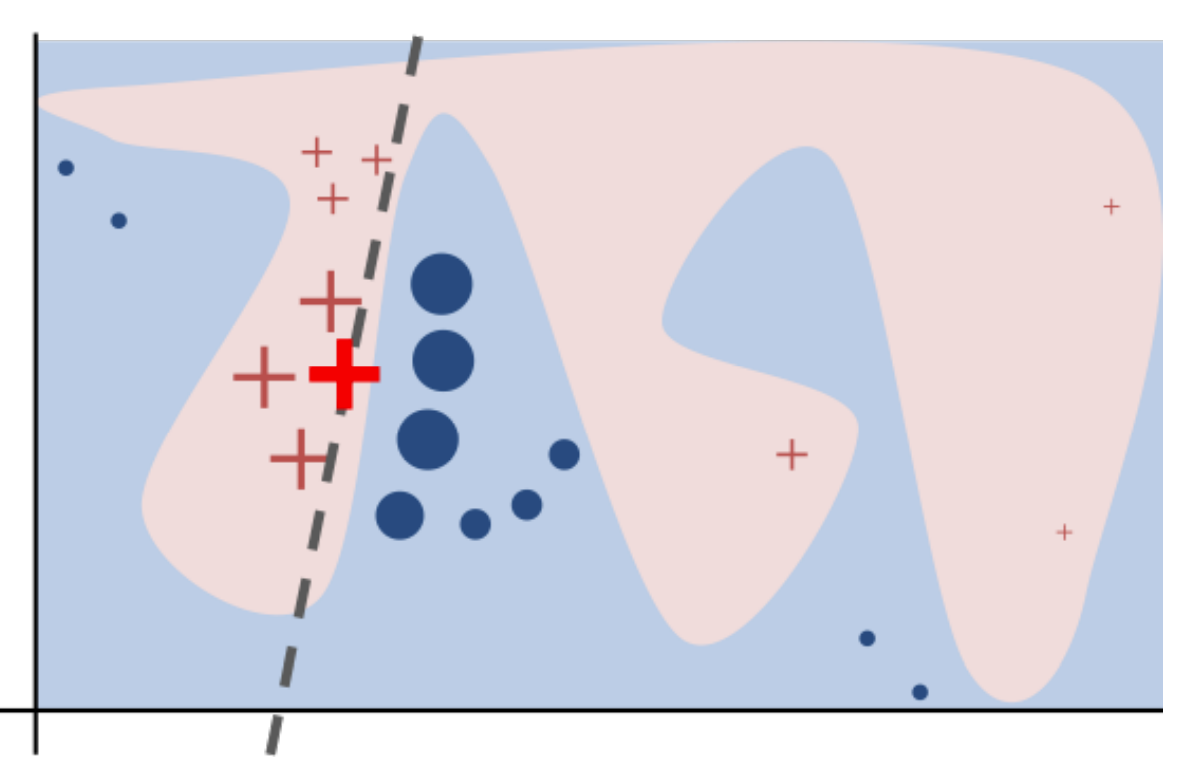
\includegraphics[width=0.4\linewidth]{lime_concept}
    \caption{(Left) Global vs (Right) Local}
  \end{figure}
\end{frame}


\begin{frame}
  \frametitle{Challenges on global methods}
  Extract an interpretable quantity that \textcolor{red}{holds for $x \in \mathcal{X}$}
  \begin{itemize}
    \item Fidelity: does the interpretable quantity mimics the model's behavior?
    \item Interpretability: is the extracted quantity interpretable enough?
    \item Can we have both?
    \begin{itemize}
      \item if yes, why not replacing the original model with an interpretable one?
      \item if no, how to deal with the trade-off?
    \end{itemize}
  \end{itemize}

  \noindent\makebox[\linewidth]{\rule{\paperwidth}{0.4pt}}
  Spoiler: Maybe uncertainty helps...
\end{frame}


\begin{frame}
  \frametitle{Methods we will discuss}

  \begin{itemize}
    \item Feature Effect
    \item Feature Interaction
    \item Feature Importance
  \end{itemize}

\end{frame}
